\documentclass[12pt, openany]{report}
\usepackage[utf8]{inputenc}
\usepackage[T1]{fontenc}
\usepackage{amsmath,amsfonts,amssymb}
\usepackage{amssymb}
\usepackage{multicol}
\usepackage[a4paper,left=2.5cm,right=2.5cm,top=2.5cm,bottom=2.5cm]{geometry}
\usepackage[english]{babel}
\usepackage{libertine}
\usepackage{graphicx}
\usepackage{wrapfig}
\usepackage{algorithm}
\usepackage{algpseudocode}
\usepackage{float}
\usepackage{enumitem}
\usepackage{pythonhighlight}
\usepackage[]{titletoc}
\usepackage{empheq}
\usepackage{titlesec}
\usepackage{mathpazo}
\usepackage{xfrac}
\usepackage{textcomp}
\usepackage{mathtools}
\usepackage{caption}
\usepackage{tabularray}
\usepackage{subcaption}
\usepackage[bottom]{footmisc}
\usepackage{pdfpages}
\usepackage{tabularx}
\usepackage{amsthm}
\usepackage{listings}
\usepackage[skins]{tcolorbox}
\titleformat{\chapter}[display]
  {\normalfont\bfseries}{}{0pt}{\Huge}
\usepackage{hyperref}
\newcommand{\hsp}{\hspace{20pt}}
\newcommand{\HRule}{\rule{\linewidth}{0.5mm}}
\newcommand{\R}{\mathbb{R}}
\newcommand{\C}{\mathbb{C}}
\theoremstyle{definition}
\newtheorem{thm}{Theorem}[chapter]
\newtheorem{definition}[thm]{Definition}
\newtheorem{lem}[thm]{Lemma}


\definecolor{mGreen}{rgb}{0,0.6,0}
\definecolor{mGray}{rgb}{0.5,0.5,0.5}
\definecolor{mPurple}{rgb}{0.58,0,0.82}
\definecolor{backgroundColour}{rgb}{0.95,0.95,0.92}

\lstdefinestyle{CppStyle}{
    backgroundcolor=\color{backgroundColour},   
    commentstyle=\color{mGreen},
    keywordstyle=\color{magenta},
    numberstyle=\tiny\color{mGray},
    stringstyle=\color{mPurple},
    basicstyle=\footnotesize,
    breakatwhitespace=false,         
    breaklines=true,                 
    captionpos=b,                    
    keepspaces=true,                 
    numbers=left,                    
    numbersep=5pt,                  
    showspaces=false,                
    showstringspaces=false,
    showtabs=false,                  
    tabsize=2,
    language=C
}

\hbadness=100000
\begin{document}
\begin{titlepage}
    \begin{sffamily}
    \begin{center}
        
\includegraphics[scale=0.25]{img/page_de_garde.png} \\[1cm]
        \HRule \\[0.4cm]
        { \huge \bfseries LINMA2710 Scientific Computing \\[0.4cm] }
    
        \HRule \\[1.5cm]
        \textsc{\LARGE Issambre L'Hermite Dumont \\ Simon Desmidt}\\[1cm]
        \vfill
        \vspace{2cm}
        {\large Academic year 2024-2025 - Q2}
        \vspace{0.4cm}
         
        
\includegraphics[width=0.15\textwidth]{img/epl.png}
        
        UCLouvain\\
    
    \end{center}
    \end{sffamily}
\end{titlepage}

\setcounter{tocdepth}{1}
\tableofcontents
\chapter{Shared-Memory Multiprocessing}
\section{How memory works}
\subsection{Memory hierarchy} 
To store the data that it will use, the CPU uses memory. Memory is hierarchical like a pyramid. The higher it is, the faster it goes, but the less space there is.
\begin{figure}[H]
    \centering
    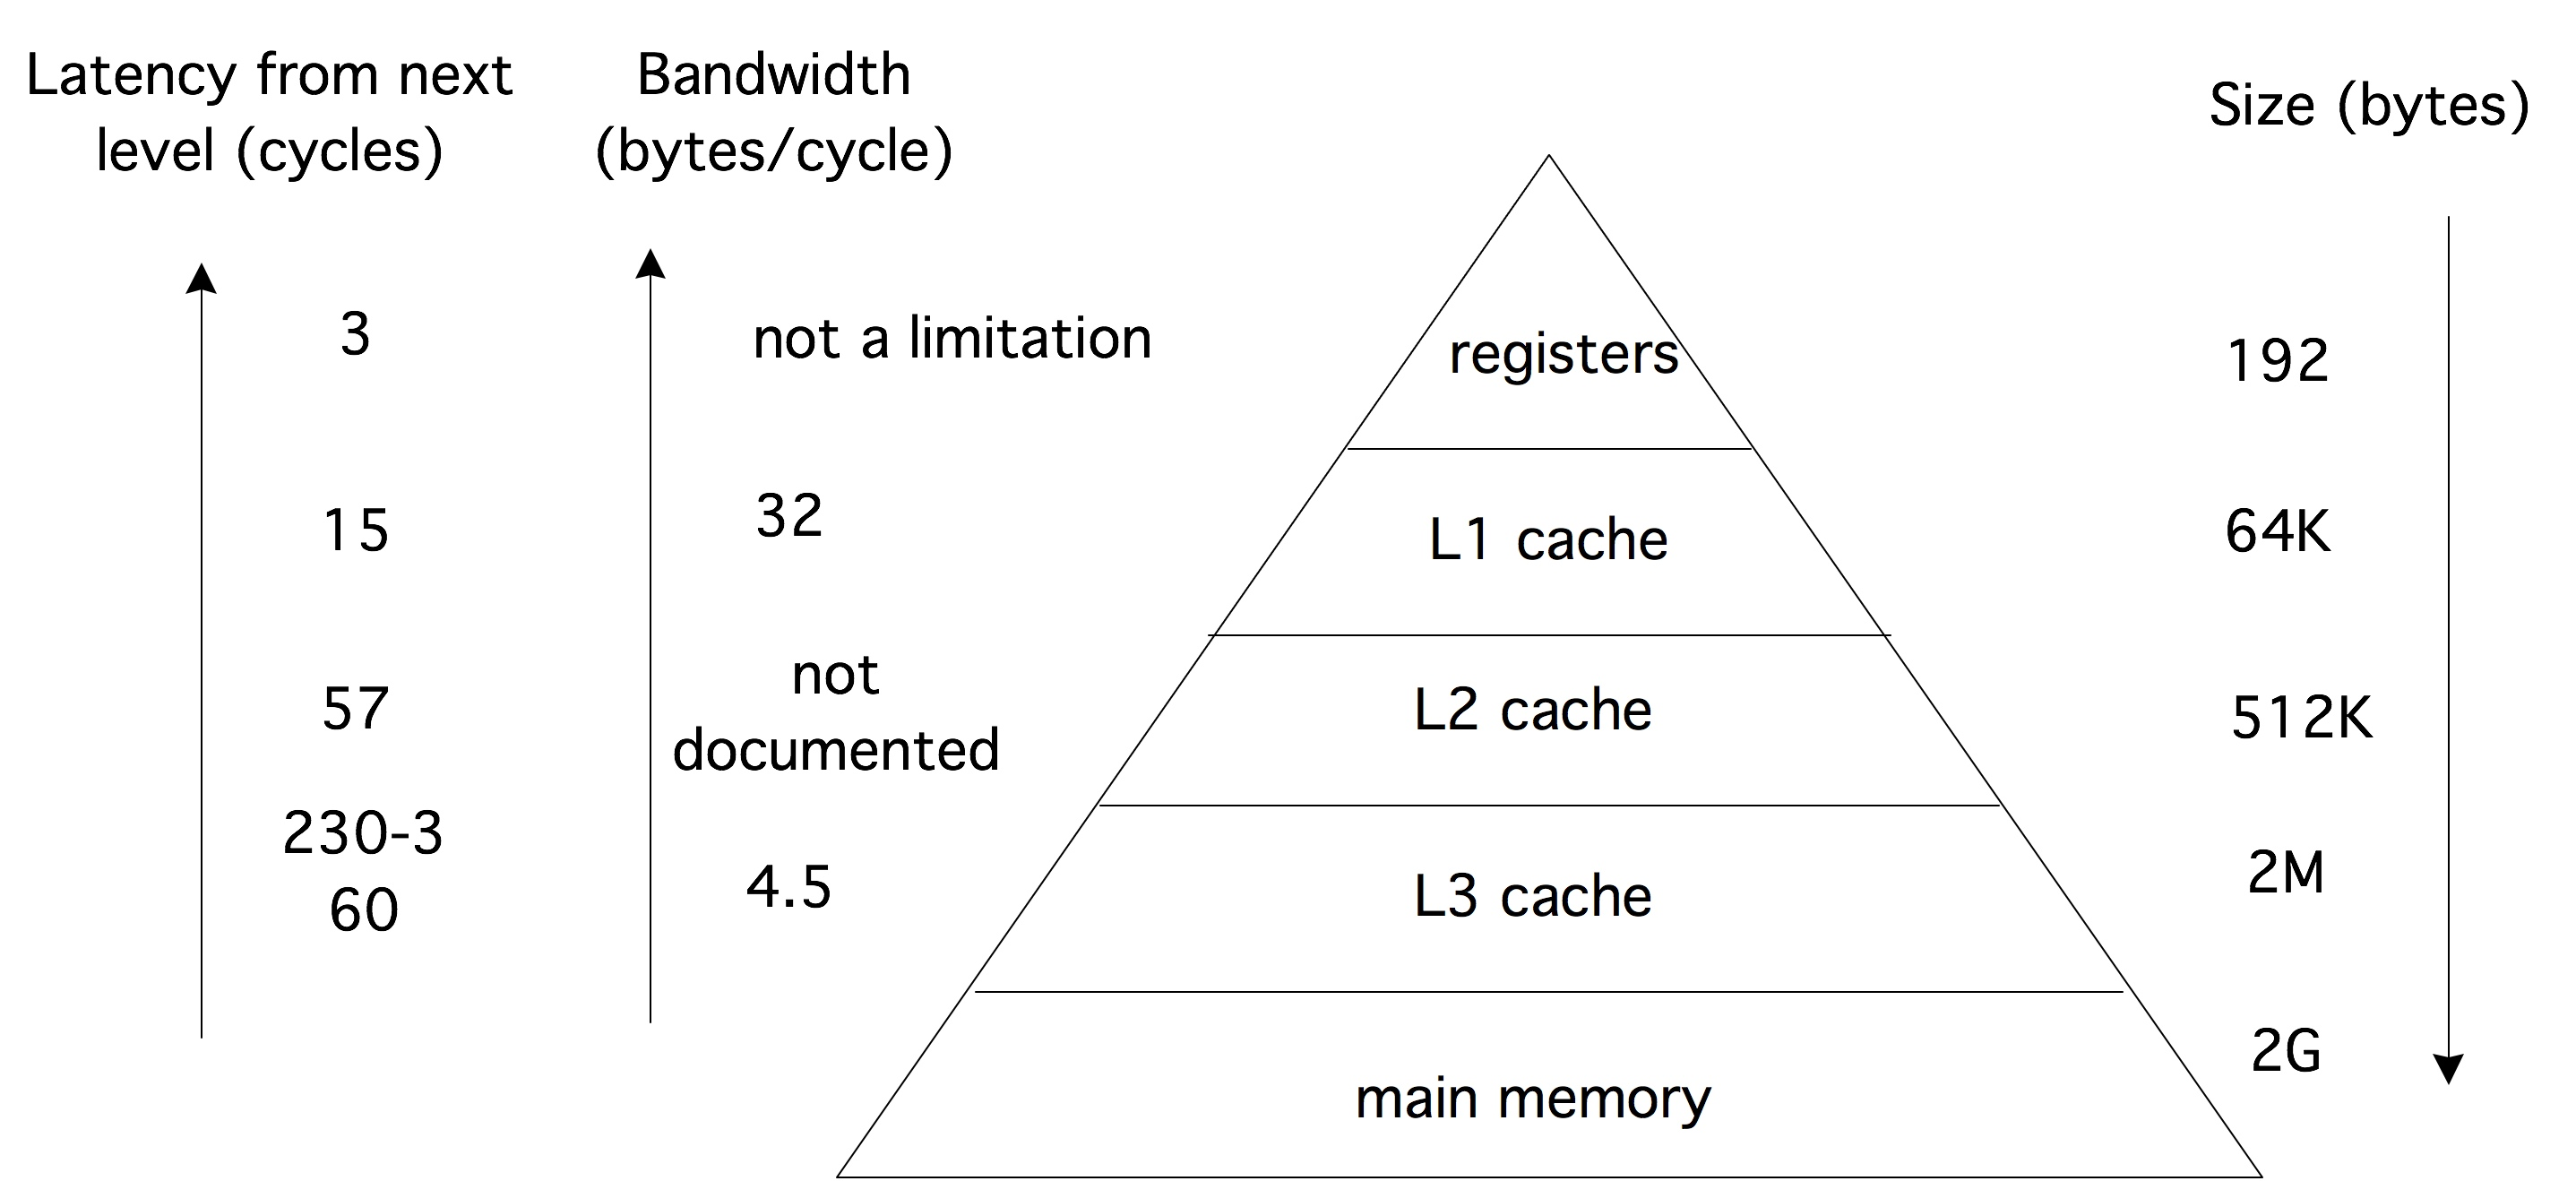
\includegraphics[scale=0.15]{img/memory_layout.jpeg}
    \caption{Memory hierarchy}
    \label{fig:memory_hierarchy}
\end{figure}
First we need to define a cycle \label{cycle_def}. It's an unit of time that is defined like this: $cycle = \frac{1}{\text{CPU freq}}$. For example, for the CPU \textit{AMD Ryzen 5 5600X}, the maximum frequency is $4.6 GHz$, so the cycle is $cycle = \frac{1}{4.6 GHz} \approx 0.217 ns$. The \textbf{bandwidth} is the number of bytes that can be transferred in one cycle. And the \textbf{latency} is the number of cycles required to access a level of memory. There's also the \textbf{latency} but for a number of bytes, its formula is $\alpha + \beta n$ where $\alpha$ is the level latency, $\beta$ is the inverse of the bandwidth and $n$ is the number of bytes.\\
\begin{tabularx}{\textwidth}{|c|X|X|X|X|X|}
	\hline
	Level & Level \newline Latency $[cycle]$  & Bandwidth $[bytes/cycle]$ & Size & What \newline is stored & example \\
	\hline
	Register & $3$ & No limit & $\pm 192B$ & "Immediate" data for the CPU & Results of addition, memory address\\
	\hline
	Cache L1 & $15$ & $32-64$ & $\pm 64KB$ & Instructions and \newline "Immediate" data & Local \newline variable\\
	\hline
	Cache L2 & $57$ & $16-32$ & $\pm 512KB$ & Data used recently & Data struct, code part\\
	\hline
	Cache L3 & $230-360$ & $4-10$ & $\pm 64MB$ & Data shared between core& Global \newline variable\\
	\hline
	RAM & $300-500$ & $9-50GB/s$ & $\geq 4GB$ & Running programs & Running software, open \newline document\\
	\hline
	Disks & $\geq 10^5$ & Usually $\leq 3GB/s$ & $\geq 128GB$ & Persistent data & Document, OS, etc\\
	\hline
\end{tabularx}
\subsection{Caches lines and prefetching}\label{caches_lines}
A \textbf{cache line} is a small fixed-size contiguous block of memory, usually $64$ or $128$ bytes. It's not necessarily stored in the cache. We use them to organize the memory, because it is easier to deal with fixed size block. When the CPU need to access a memory location, it loads the entire cache line into the cache of the CPU.
If the wanted data is not in the cache, there will be a \textbf{cache miss}. After that the CPU will load the entire cache line into the cache.\\
The \textbf{prefetching} is the fact that the CPU will load the cache line that is next to the one that is needed. It's because of the spacial locality. Spacial locality is the reason why we use cache lines. For example, if we store an array of data, it may use some space greater than one cache line so for precaution, the CPU will load the next cache line too. And so we save time, by anticipating.\\
The data locality is important for at least the two following reasons:
\begin{itemize}
	\item \textbf{Temporal locality}: If a data is used frequently, we will keep it in the cache.
	\item \textbf{Spacial locality}: If a data is used, the data next to it could be useful too.
\end{itemize}
\newpage
\subsection{Arithmetic intensity}
The \textbf{arithmetic intensity} is a concept in performance analysis for memory-bound and compute-bound programs.
Let's consider a program that does $o$ arithmetic operations and $m$ memory operations, we define:
\begin{itemize}
	\item \textbf{Arithmetic intensity}: 
	\begin{equation} 
		a = \frac{o}{m}
	\end{equation}
	It helps to find if the program is limited by a compute-bound or memory-bound.
	\item \textbf{Arithmetic time}: 
	\begin{equation} 
		t_{arith} = \frac{o}{\text{CPU freq}}
	\end{equation}
	It's the time needed to perform $o$ operations.
	\item \textbf{Memory transfer time}:
	\begin{equation} 
		t_{mem} = \frac{m}{\text{bandwidth}} = \frac{o}{a \times \text{bandwidth}}
	\end{equation}
	It's the time needed to do $m$ memory operations. 
\end{itemize}
The overall performance of a program is thus defined by the worst component of the PC, and so we get the \textbf{time per iteration}:
\begin{equation}
	\min \left( \frac{t_{arith}}{o},\frac{t_{mem}}{o} \right)
\end{equation}
With some algebra, we can find the \textbf{number of operations per second}:
\begin{equation}
	\max \left( \text{CPU freq}, a \times \text{bandwidth} \right)
\end{equation}
To resume:
\begin{itemize}
	\item If $a$ is low then the performance is memory-bounded $\Rightarrow$ \textbf{Need cache optimization}.
	\item If $a$ is high then the performance is compute-bounded $\Rightarrow$ \textbf{Need more CPU cores or vectorization}.
\end{itemize}
The arithmetic intensity can be represented with the \textbf{roofline model} which we'll talk now.
\newpage
\subsection{The roofline model}
The two following graph link the performances of a program with the arithmetic intensity. The "performances" means the number of operations per second and the "arithmetic intensity" is the number of operations per byte of memory transferred. The right graph is the case where we consider a perfect usage of the PC, and the left graph is the case where we consider a bad usage of the PC.  
\begin{figure}[H]
	\begin{subfigure}[b]{0.45\textwidth}
		\centering
		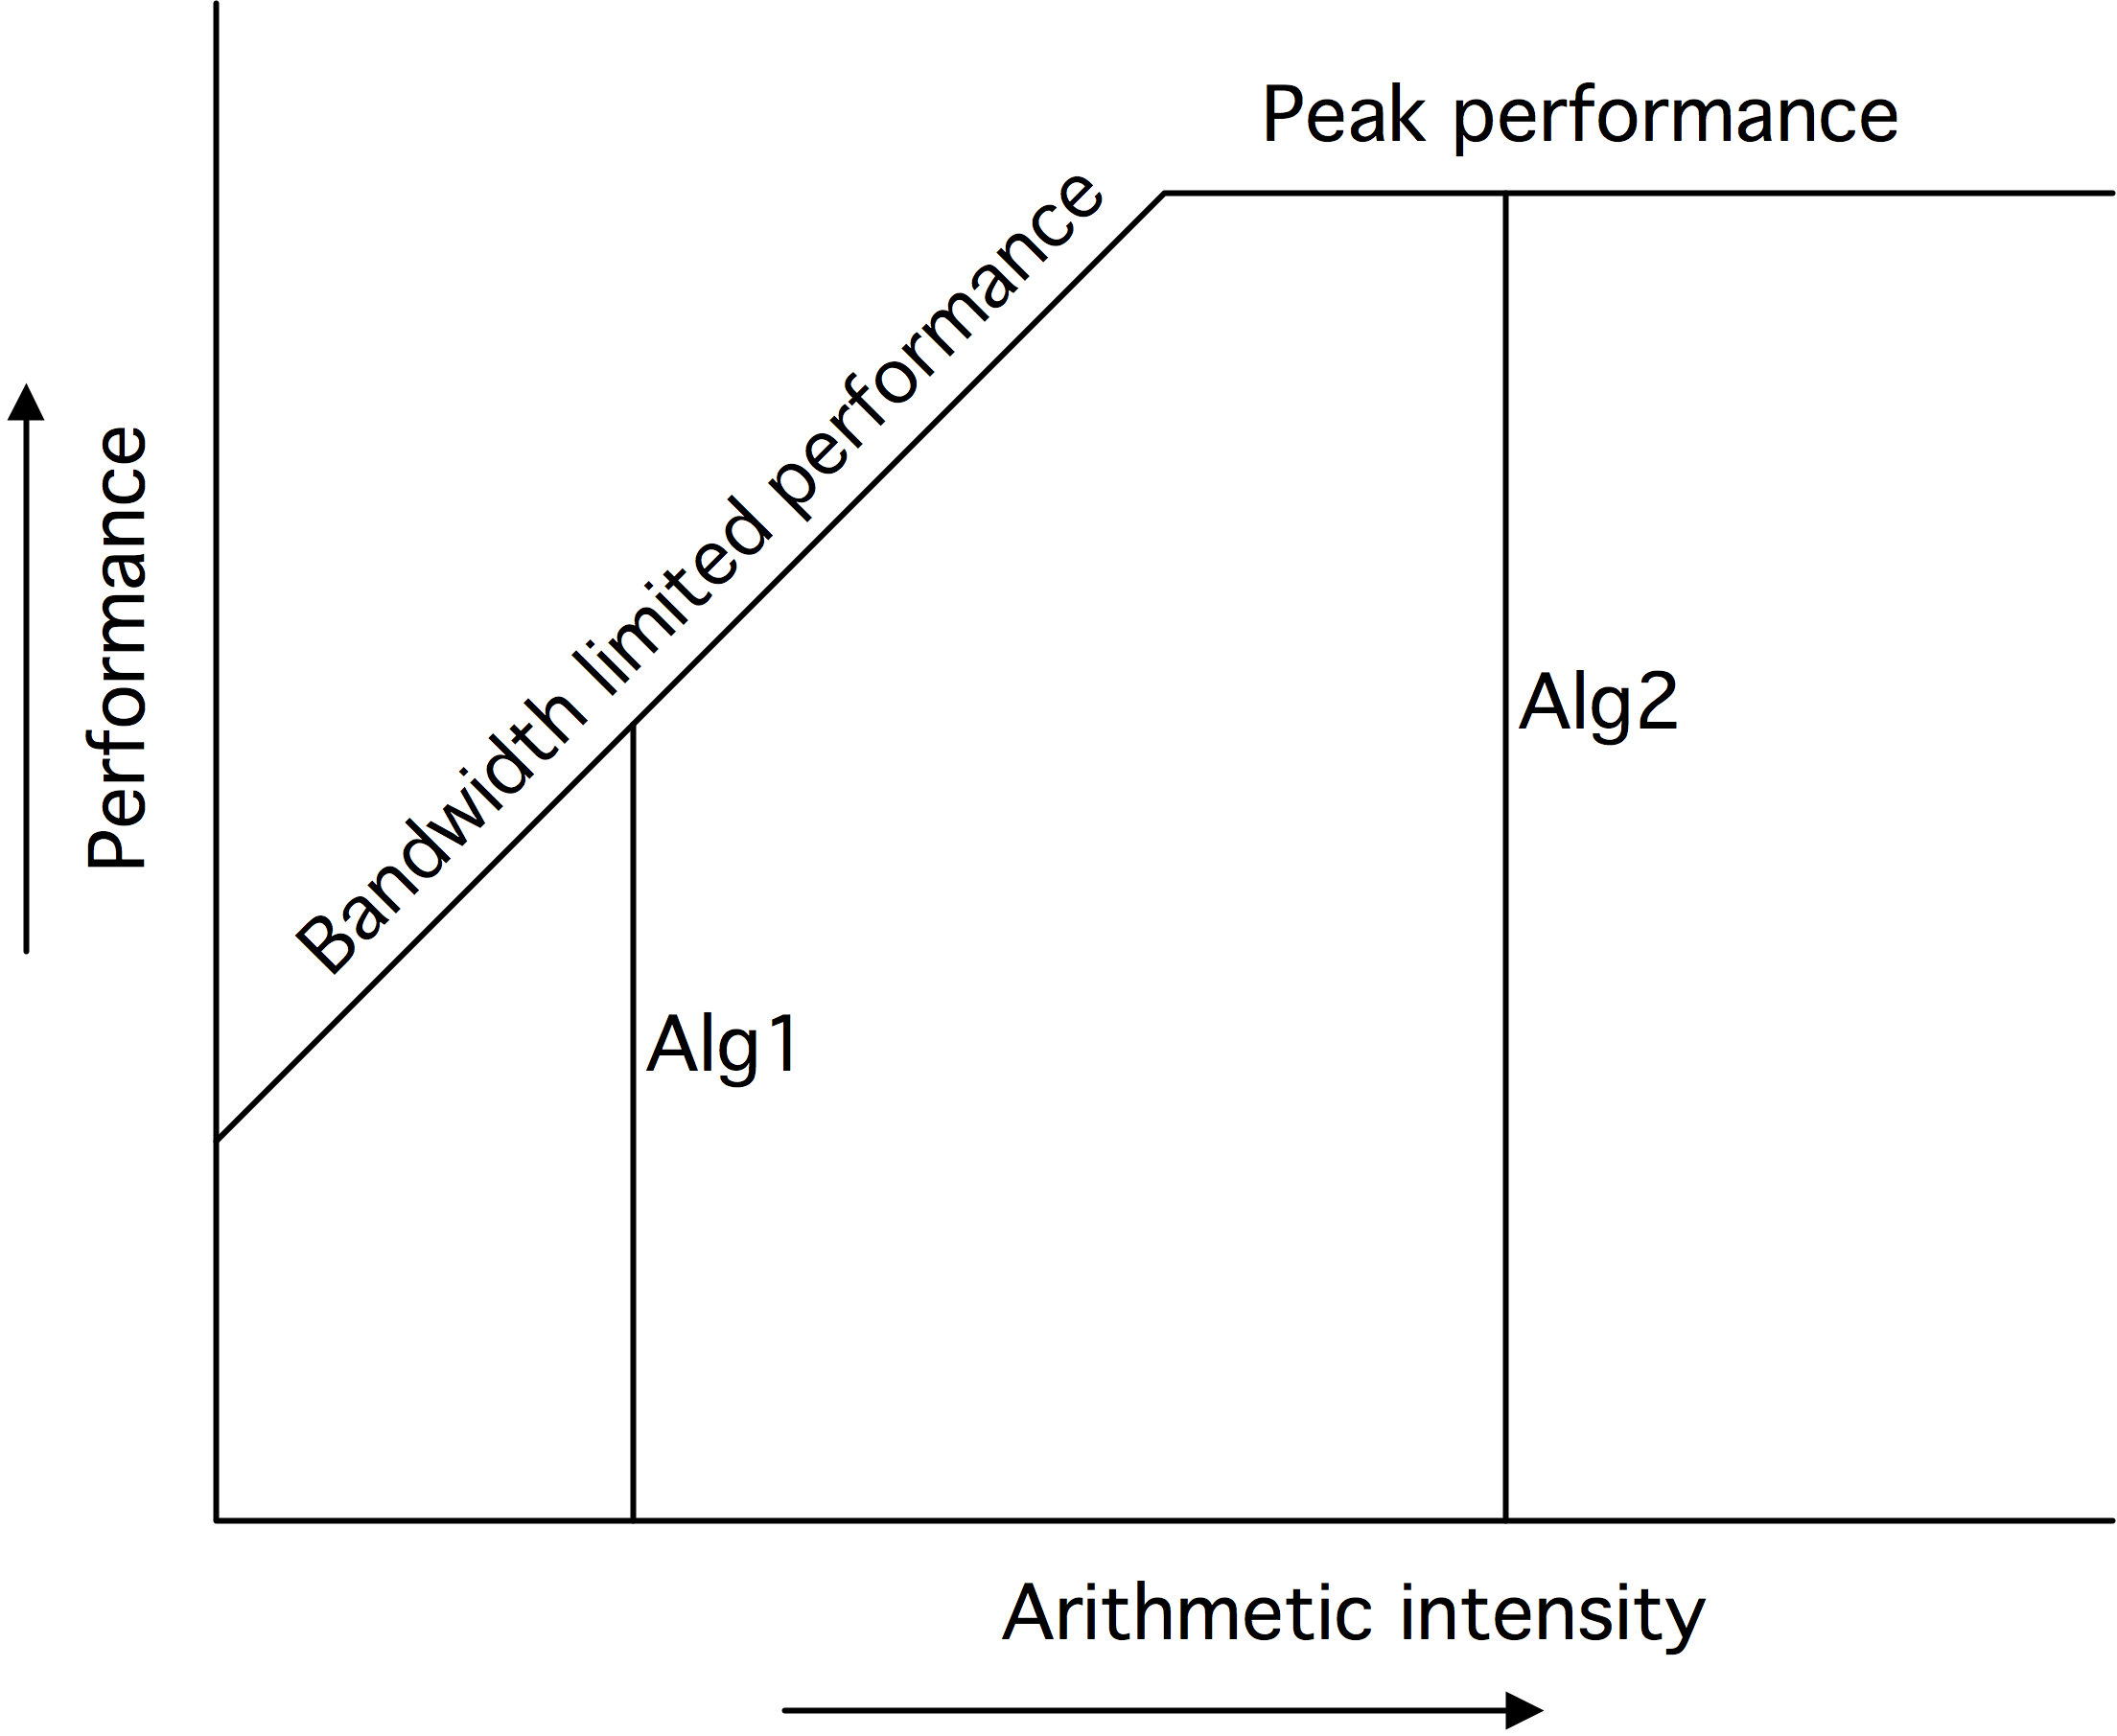
\includegraphics[scale=0.10]{img/roofline.jpeg}
		\caption{Roofline model}
		\label{fig:roofline}
	\end{subfigure}
	\begin{subfigure}[b]{0.45\textwidth}
		\centering
		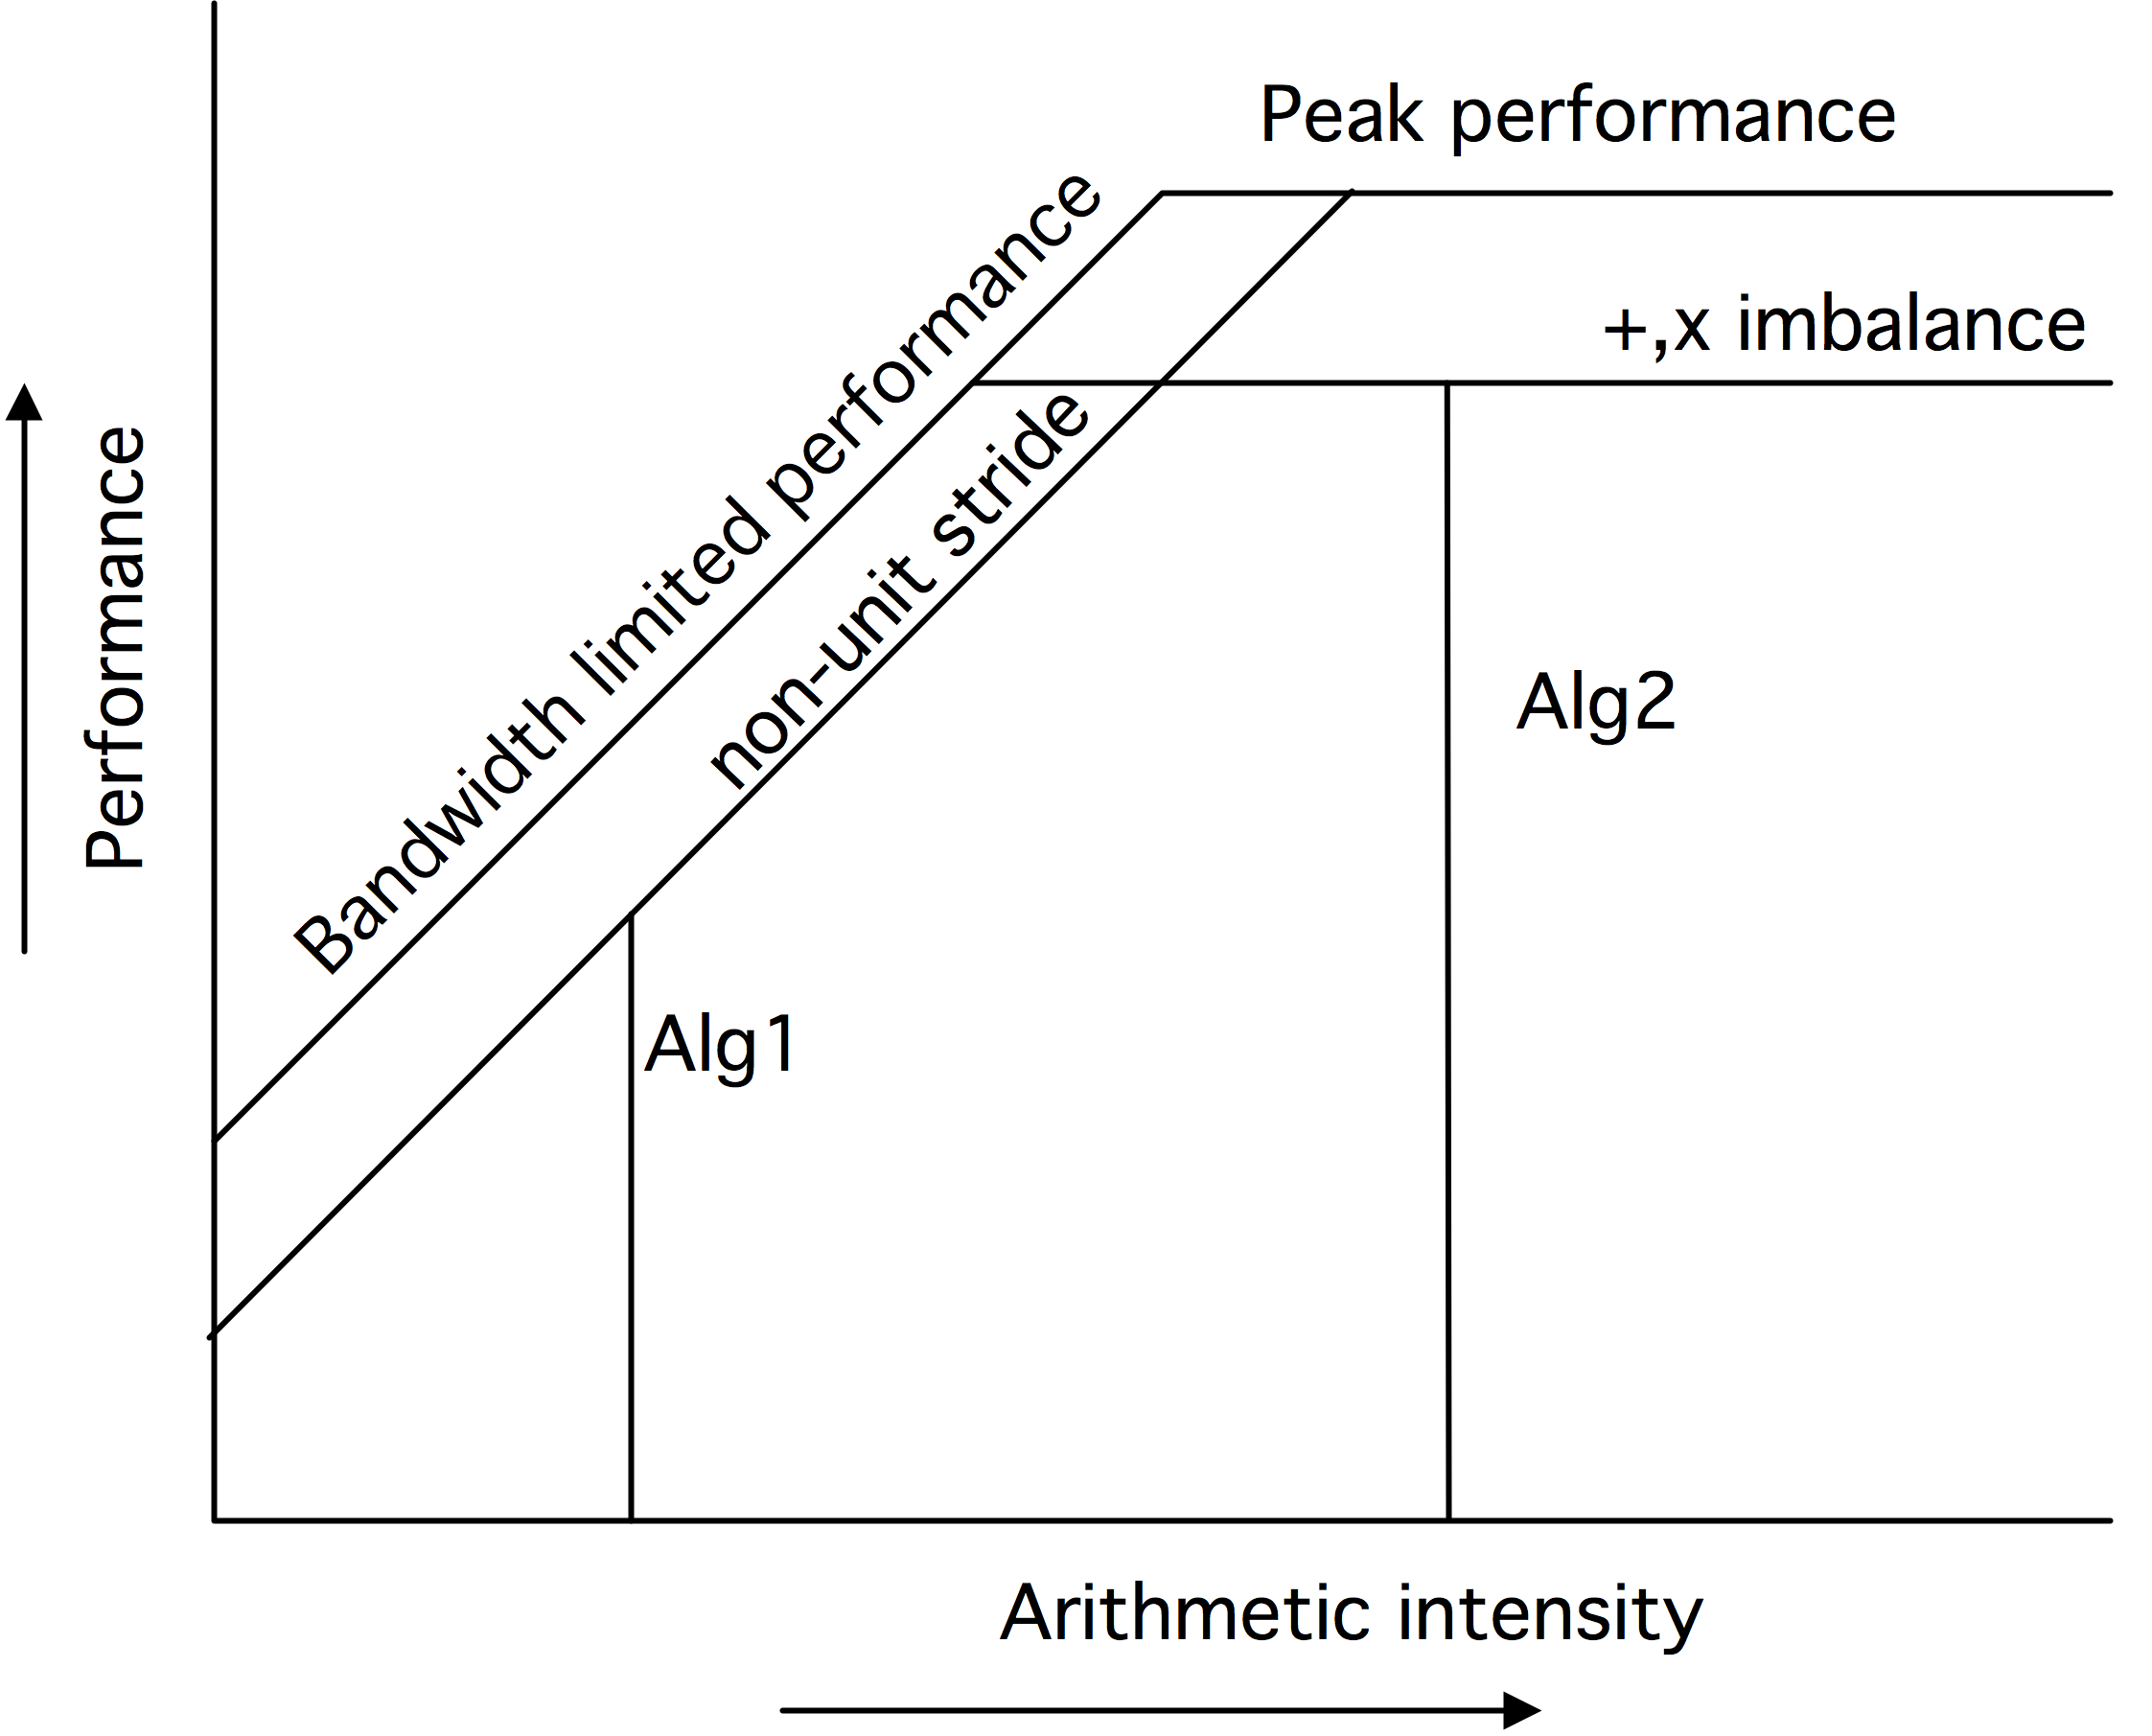
\includegraphics[scale=0.10]{img/roofline2.jpeg}
		\caption{Model with worse performances}
		\label{fig:roofline2}
	\end{subfigure}
\end{figure}
As we can clearly see, we have two limitations:
\begin{itemize}
	\item Bandwidth limit (slopped line)
	\item Computing limit (flat line)
\end{itemize}
These two limits lines are upper bound for performances and are limited from above by the hardware (we can't do better than what our CPU can do), but they can be lower if the program is not optimized. For example the slopped line can be lower if we don't use the cache correctly. The flat line can be lower if we don't use the CPU correctly (e.g. using SIMD).\\
\newpage
\subsection{Cache hierarchy for a multi-core CPU}
In the case where we have a multi-core CPU, the organization of the memory isn't always the same, it depends of the CPU architecture. For example, we can have a hierarchy like this:
\begin{figure}[H]
	\centering
	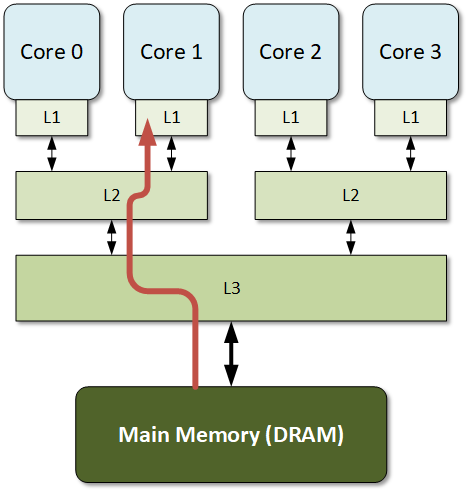
\includegraphics[scale=0.5]{img/multicore-cache.png}
	\caption{Cache hierarchy for a multi-core CPU}
	\label{fig:multi_core_cache}
\end{figure}
Here the L1 cache is private to each core, the L2 cache is shared between two cores and the L3 cache is shared between all cores, as well as the RAM. 
\section{Parallelism}
In this course, we use \textit{OpenMP} to parallelize our code instead of \textit{lpthread}. The advantages of \textit{OpenMP} are detailed in the chapter \textbf{useful tools} at the section \ref{OpenMP}.\\ 
Parallelism is a very useful tool to optimize the performances of a program. It allows to use multiple cores of the CPU to do multiple tasks at the same time. But sometimes it may arise some problems of performances or computational error.
\subsection{computational error}
When using multi-threading, we may modify and use some variables at the same time which could cause computational error. So to avoid that we can either protect the variable (with some adapted tools) but this option is not very efficient because it takes some time to \textit{lock} and \textit{unlock} and to wait for the variable to be available. Or we can make each thread use its own version of the variable, this introduces the next problems.
\subsection{Race condition}
The race condition is a problem that occurs when two or more threads try to modify the same variable at the same time, here there are no computational error possible. For example if all the threads want to modify a variable a the same time, they will need to wait for the variable to be available, and it is a waste of time. The solution for that, as we said before is to make each thread use its own version of the variable. Let's say they need to compute the sum of an array. The solution is to make each thread compute the sum of a part of the array and then by "reduction" sum all the sums. We will see this in more detail in the next chapter.
\subsection{False sharing}
As we say before, in the section about cache lines \ref{caches_lines}, the CPU loads the entire cache line into the cache when it need to use some data that is on the cache line. So here is the problem, let's say that all of the partial sum of the array are stored in the same cache line, when a thread modify its partial sum, the entire cache line is loaded into the cache of the CPU, and so the other threads will have to wait for the cache line to be available. The solution is to make each thread use its own cache line. We can solve this by adding some padding (shift the data) to the data structure.
\section{Amdahl's law}
First let's define the \textbf{speedup} of a program, it represents the improvement of running time while using $p$ threads. It is defined by:
\begin{equation}
	S_p = \frac{T_1}{T_p}
\end{equation}
Where $T_1$ is the time needed to run the program with one thread and $T_p$ is the time needed to run the program with $p$ threads.\\
Then let's define the \textbf{efficiency} of a program, is mesures how well the parallelization is done. It is defined by:
\begin{equation}
	E_p = \frac{S_p}{p}
\end{equation}
Where $S_p$ is the speedup of the program with $p$ threads. We get 3 cases:
\begin{itemize}
	\item If $E_p = 1 \Rightarrow$ \textbf{Ideal case}, the parallelization is perfect.
	\item If $E_p < 1 \Rightarrow$ \textbf{Realistic case}, there's some inefficiency.
	\item If $E_p > 1 \Rightarrow$ \textbf{Unrealistic case}, would imply a super-linear speedup.
\end{itemize}
We can now define \textbf{Amdahl's law}, which explain the limitation of parallelization due to the presence of a sequential portion in a program. It is defined like this:
\begin{equation}
	T_p = F_sT_1 + \frac{(1 - F_s)T_1}{p}
\end{equation}
$F_s$ is the percentage of the program that is sequential (impossible to parallelize). With that we can redefine the \textbf{speedup} and the \textbf{efficiency} of a program:
\begin{equation}
	S_p = \frac{T_1}{F_sT_1 + \frac{(1 - F_s)T_1}{p}} = \frac{1}{F_s + \frac{1 - F_s}{p}} \Rightarrow \lim_{p \to \infty} S_p = \frac{1}{F_s}
\end{equation}
And
\begin{equation}
	E_p = \frac{S_p}{p} = \frac{1}{pF_s + 1 - F_s} = \frac{1}{F_s(p - 1) + 1}
\end{equation}
\subsection{Application of Amdahl's law to parallel sum}
Let's consider the sum of an array, we want to parallelize it. The time without parallelization is $n$ and with parallelization is $\frac{n}{p} + \log_2(p)$, the log term is the time needed to sum all the partial sums. So the speedup is:
\begin{equation}
	S_p = \frac{n}{\frac{n}{p} + \log_2(p)} = \frac{1}{\frac{1}{p} + \frac{\log_2(p)}{n}}
\end{equation}
And the efficiency is:
\begin{equation}
	E_p = \frac{S_p}{p} = \frac{1}{1 + \frac{p}{n}\log_2(p)}
\end{equation}
We clearly see that if we use more than $n$ processes the efficiency will decrease. Because if $p \geq n$ then we have $T_p = \log_2(n)$ and $\lim_{s \to \infty} S_p = \frac{1}{\log_2(n)}$ and $F_s = \log_2(n)$
\chapter{Single Instruction Multiple Data (SIMD)}
\textcolor{red}{Maybe to improve}\\
SIMD (Single Instruction Multiple Data) is a parallel computing architecture used to process multiple data points simultaneously with a single instruction.\\
The idea of SIMD is that instead of executing the same instruction separately for each data element, SIMD processes multiple elements in parallel within a single CPU cycle. To simplify SIMD takes advantages of \textbf{vectorization}, to optimize the performances of the program. It uses register to store the vector on which it does the computing.\\
Let's do a little example, consider the following code:
\begin{lstlisting}[style=CppStyle]
	int a[] = {...};
	int b[] = {...};
	int c[size];
	for(int i = 0; i < size; i++)
		c[i] = a[i] + b[i];
\end{lstlisting}
Here we use \texttt{int} which is $32$ bytes so if we use SIMD with AVX2 registers, we can store $(512/32 =) 16$ integers in a register. And so SIMD with that type of registers will automatically translate the previous code to:
\begin{lstlisting}[style=CppStyle]
	int a[] = {...};
	int b[] = {...};
	int c[size];
	for(int i = 0; i < size; i+=16)
    __m512_add_epi16(c + i, a + i, b+i);
\end{lstlisting}
We can write the code with the intrinsics (\texttt{\_\_m512\_add\_epi16}) but it's not necessarily. The compiler will do it for you.\\
To use SIMD, you need to give to your compiler some flags, for example:
\begin{itemize}
	\item \texttt{-O2} or \texttt{-O3} for optimization
	\item \texttt{-mavx} for AVX
	\item \texttt{-mavx2} for AVX2
	\item \texttt{-mavx512} for AVX512
\end{itemize}
\chapter{Distributed Computing with MPI}
\section{Single Program Multiple Data (SPMD)}
Single Program Multiple Data means that we make multiple processes execute the same program but operate on different data. It's a kind of parallel computing.
\section{Collectives}
\begin{figure}[H]
	\centering
	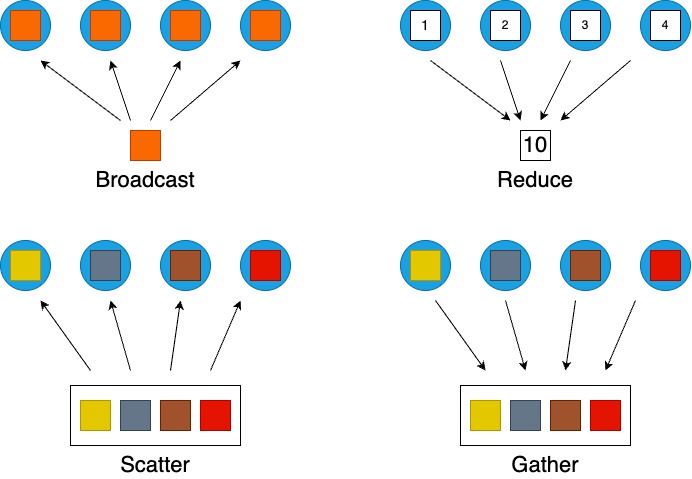
\includegraphics[scale=0.5]{img/collectives.jpeg}
	\caption{Collectives}
	\label{fig:collectives}
\end{figure}
\subsection{Broadcast}
\subsection{Gather}
\subsection{Reduce}
\subsection{All gather}
\subsection{Reduce scatter}
\chapter{Useful tools}
\section{OpenMP}\label{OpenMP}
\textcolor{red}{TODO: Improve}\\
\textit{OpenMP} is a library that allows to parallelize code, it is better than \textit{lpthread} for multiple reasons:
\begin{itemize}
	\item Easy to add to an existing code, because of the compilation directives (\texttt{\#pragma omp}). It's an implicit gestion of the threads unlike \textit{lpthreads} that require an explicit gestion. It allows to parallelize a code without changing the whole structure of the code.
	\item Automatic gestion of the threads, for example if you want to parallelize a loop, you don't have to create the threads, the library will do it for you and optimize the number of threads.
	\item Simplified synchronization with tools. \textit{OpenMP} provides tools to synchronize the threads like \texttt{critical}, \texttt{atomic}, \texttt{barrier}, etc. They help to protect the shared data between the threads.
	\item Optimized use of the cache
	\item Compatible with \textit{SIMD}
	\item Portability: it is compatible with \textit{Windows}, \textit{Linux}, \textit{MacOS}. With multiple CPU architectures like \textit{Intel}, \textit{AMD}, \textit{ARM}, etc.
\end{itemize}
\end{document}